\documentclass[../main.tex]{subfiles}


\begin{document}
\raggedright
Django is a Python based web framework which allows clean and pragmatic design as well as rapid development. The framework is designed to enable the coders to code without worrying about the security of the code as it guides the coders through securing the vulnerabilities such as SQL injection, cross-site scripting, cross-site request forgery and clickjacking. Django also has a user authentication system which can be customised to allow a secure way for data to be transferred\cite{django}. Not only does Django provide security, it also allows efficient and easy coding as it follows the model, controller view system which avoids repeated code. With Python being the main language, numerous frameworks are available to make working with Django even easier.\cite{whyusedjango} 

\subsection{Django vs Laravel}
Django is Python based as stated above but Laravel\cite{laravel} on the other hand is a PHP based web framework. Django follows the Model View template similar to Ruby on Rails but Laravel follows Object Oriented Programming as well as the Model View Template. In terms of website security, Django takes it extremely seriously and helps developers avoid the common mistakes which lead to the website having vulnerabilities while Laravel also has a guide to avoid making such mistakes but its contents are not as informative and detailed as Django. You would need to manually test each of the security features unlike Django where the system makes sure that all security protocols are in place with latest updates.
Django is naturally very fast as it uses Python which is known for its speed and processing. Djano beats Laravels speed in all; Plaintext, JSON and SQLite Fetch\cite{djangovslaravel} as shown in Figure \ref{fig:djangovslaravelsp}.

\begin{figure}[H]
        \center{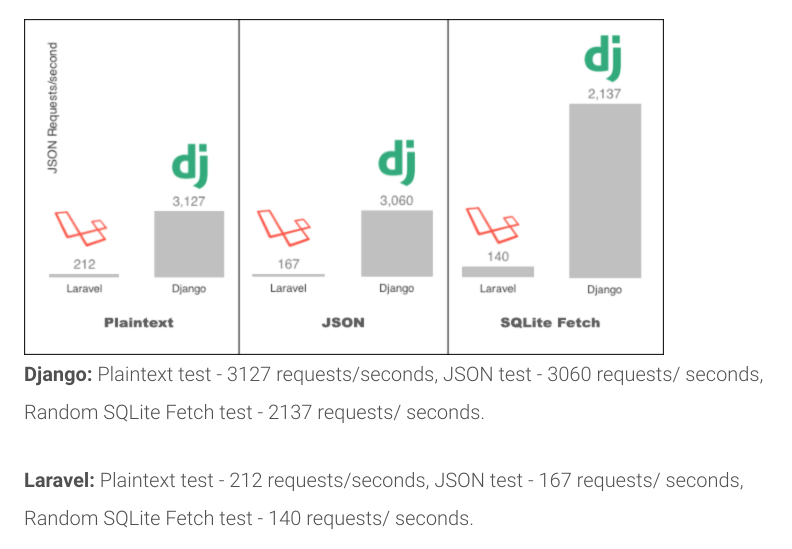
\includegraphics[scale=1]
        {images/djangovslaravelspeeds.png}}
        \caption{\label{fig:djangovslaravelsp} Django vs Laravel Speeds 2016 - CabotSolutions\cite{djangovslaravel}}
      \end{figure}
      
      
\subsection{Django vs Ruby on Rails} 
Both are popular web frameworks, Django more than Ruby on Rails for professional developers. They are open-source which allows all code to be customised in any way. Ruby on Rails allows the use of gems which are designed by other users, these come in handy when programming personal or individual projects however with professional projects licensing is a good idea to allow the code to be usable in the future\cite{djangovsrails}. Django on the other hand has user coded packages which can be used with the application being created. An example would be \textit{django-pgcrypto}\cite{dbencrypt} which allows the encryption of database entries. 

Based on JetBrains research\cite{pythonresearch2018}\cite{rubyresearch2018} we know that Python is a really popular language compared to Ruby and it is highly used for Data Analysis and Web Development among various other things while developers use a mixture Ruby Versions which makes future updates to the code harder. Table \ref{tab:djangovsruby} shows the differences between Django and Ruby on Rails

\bgroup
\def\arraystretch{1.1}%  1 is the default, change whatever you need
\begin{table}[H]
\centering
\begin{tabular}{|l|l|l|}
\hline
& Django                                                                                                                                           & Ruby on Rails                                                                                                     \\ \hline
Pros       
& \begin{tabular}[l]{@{}l@{}}- Python is versatile \\ - Fast\\ - Caching System\\ - Data Analysis\\ - Great Security and \\ Autentication\end{tabular} 
& \begin{tabular}[l]{@{}l@{}}- Flexible\\ - Large Community\\ - Gems Available\\ - Easy Migration\end{tabular}      \\ \hline
Cons       
& \begin{tabular}[l]{@{}l@{}}- Hard to debug\\ - Monolithic architecture\end{tabular}                                                                   & \begin{tabular}[l]{@{}l@{}}- Bloated\\ - No Data Analysis\\ - Very explicit and \\ inelegant to read\end{tabular} \\ \hline
\end{tabular}
\captionof{table}{Django vs Ruby on Rails Pros and Cons \cite{djangovsrails}}\label{tab:djangovsruby} 
\end{table}
\egroup

\subsection{Django vs NodeJS} 
NodeJS\cite{nodejs} uses C, C++ and JavaScript to build the web application. The use of JavaScript mainly is extremely good when it comes to the design and feel of the web system but not when it comes to security. NodeJS can be used to produce a progressive web application which will make the website feel and work like a smart application even when there is no network as well as work perfectly on larger screens too. However, being that security is an important requirement for our system, Django would win over NodeJS\cite{nodejsdjango}

\subsection{Security}
A paper on Web Development Done Right\cite{Holovaty2007TheDG} has considered Django's security as well as all other aspects to build a secure web based application in Django. According to the research, attackers simply need to find a single flaw in the system and they would gain access to almost everything. Django allows mitigating this difficulty and prevents most of the common mistakes that coders make. The paper numerous security attacks such as SQL Injection, Cross-site Scripting, Session Forging, Email Header Injection, Directory Traversal, Exposed Error Messages and more with solutions on how Django can prevent each of them. Overall Django's security has been appreciated by a great number of professional coders. 

\end{document}
